\chapter{Optical Coherence Tomography}

\label{optical_coherence_tomography}
\lhead{\emph{Optical Coherence Tomography}}

Optical Coherence Tomography (OCT) is an important advancement in retinal imaging technology.  Research leading to OCT technology was made possible during the 1980’s with “advances in the fiber-optics and photonics industries” and was eventually developed in 1991 by David Huang and colleagues.\cite{mbib_1,mbib_2,mbib_3}  Since 1991, many improvements have been made to enable high quality and detailed scans of retinal tissues.  The retina, as mentioned previously, is made up of twelve internal layers with a total thickness between 300-500 $\mu m$.\cite{mbib_4} These layers are important indicators for monitoring and diagnosing retinal diseases, which is why opticians use technologies such as OCT to image retinal tissues.

OCT is a non-invasive imaging technique “analogous to ultrasound,” relying on low coherence (also referred to as “white light”) interferometry to generate cross-sectional imagery (or tomography) of retinal tissues within the eye to a “micrometer axial resolution” of 1-15 micrometers.\cite{mbib_5, mbib_6,mbib_2} Unlike a normal camera, which only has transverse dimensional resolution, OCT imaging uses low coherence interferometry to estimate “the depth at which a specific backscatter [from the source of light] originated.” \cite{mbib_4}  In other words, OCT images depth as opposed to simply taking an image of the surface.  Depth resolution can be carried out using three main methods: Time-domain OCT (TD-OCT), Fourier-domain OCT (FD-OCT) and Spectral-domain OCT (SD-OCT).  The latter two are normally combined as they are very similar methods, therefore for simplicity and consistency they will jointly be referred to as Spectral-domain OCT (SD-OCT).

In the following sections the physics behind OCT technology will be explained further and the different methods will be described as well as a discussion on image analysis for different purposes.

\section{Low Coherence Interferometry}
Because the velocity of light is much larger than that of the
distance between the retinal layers, “it is not possible to
measure the flight-time change directly.” \cite{mbib_5} Meaning,
the incoming and outgoing light cannot be differentiated without
the use of low coherence interferometry. Low coherence interferometry
is just as it sounds.  A low coherence light beam, which can be thought
of as a “train of highly autocorrelated overlapping ‘bursts’ of light,”
is directed at a sample surface using an optical probe, which is connected
to the interferometer.\cite{mbib_4}  When the light “burst” hits the
transparent sample, light will be reflected off of the layers within
the sample and its “unique autocorrelogram” will be detected by its
“autocorrelation function” to get an idea of the structure of the sample.
\cite{mbib_4,mbib_3,mbib_6} It should be noted that these “bursts” are a
way of explaining what is happening, and are not to be thought of as a
pulsed light source.

In \fref{fig:m_1}, a schematic of the low coherence interferometer used in the classic and current OCT imaging can be found.

\begin{figure}[htbp]
\centering
 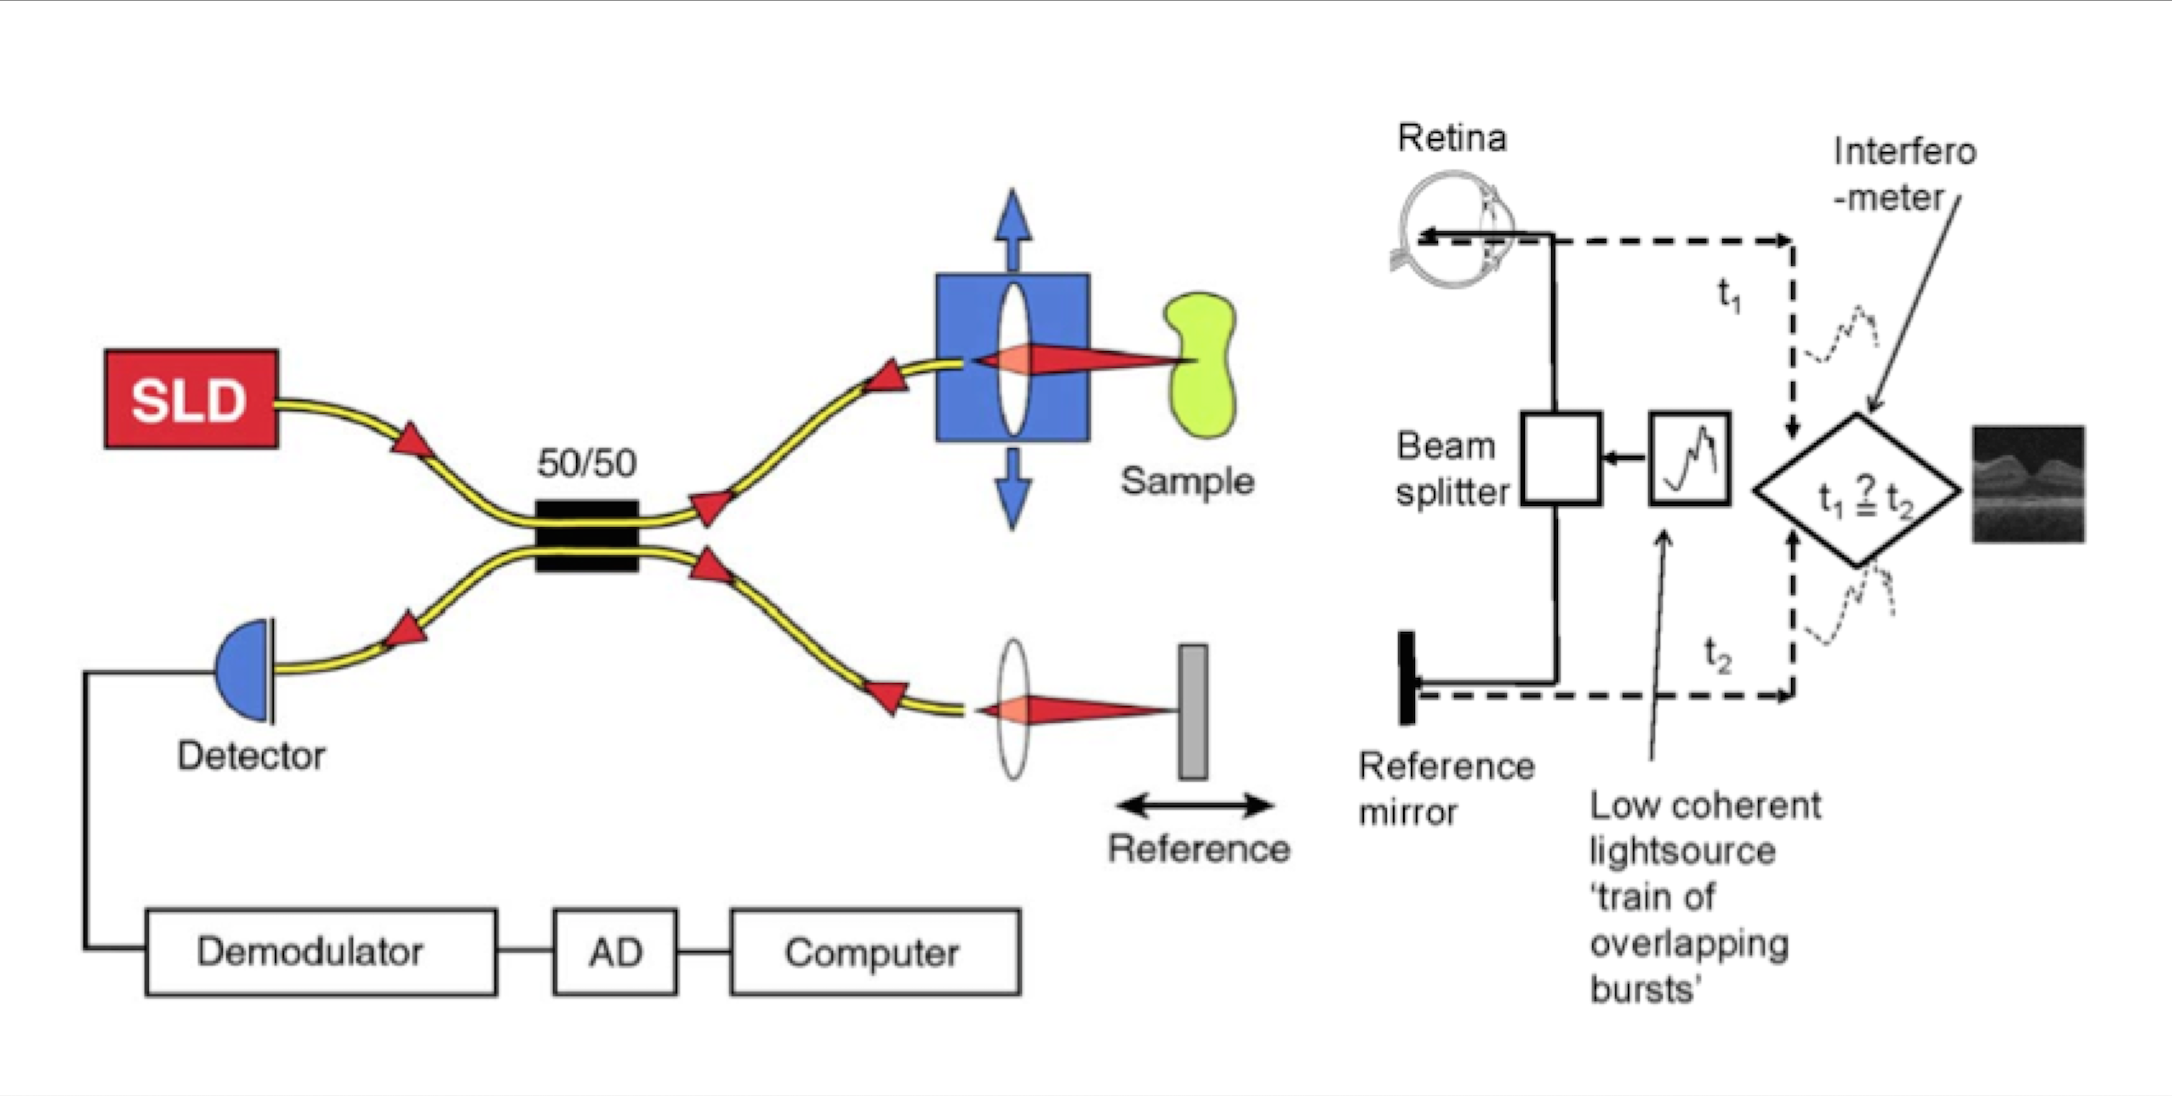
\includegraphics{figures/morgan_1}
\caption{(Left) “Schematic of the classic optical coherence
tomography system.”  (Right) “Schematic diagram of OCT, with
emphasis on splitting of the light, overlapping train of labelled
bursts based on their autocorrelogram, and their interference
after being reflected from retinal tissue as well as from the
reference mirror (assuming the time delays of both paths are equal).” \cite{mbib_6,mbib_4} }
\label{fig:m_1}
\end{figure}


Super-luminescent LEDs (SLED), also known as super-luminescent diodes (SLD),
which produce wavelengths which reside in the near infrared region, are
traditionally used in OCT interferometry because they are “economical,
compact, long-lasting, and emit high quality beams that couple efficiently
with an optical fiber.” \cite{mbib_6} Also, the amount of light coherence
is inversely proportional to the depth resolution, thus wavelengths longer
than visible light, “typically 800–1400nm wavelength in the near infrared,”
are necessary as they penetrate deeper into the retinal tissue layers.\cite{mbib_4,mbib_7}
The resolution of the images generated is limited by the progress of SLD
technology, for example, early systems used SLDs emitting wavelengths around
820 nm, limiting the axial resolution to 11 mm in retinal tissues and 15 mm
in air. \cite{mbib_6}  Today, the CirrusTM HD-OCT device uses SLDs with wavelengths
of approximately 840 nm, and achieve a resolution of 5 mm in retinal tissue. \cite{mbib_7}

Inside the interferometer, the light from the SLD is split using a beam splitter.
Other splitting methods such as a 50/50 fiber coupler can be used, but the beam
splitter is the most commonly used method to date.  When the light from the SLD
is split, half of the light is directed to a reference reflective mirror at a
specific distance, while the other is directed into the retinal tissues (sample)
using an optical fiber.  The returning beams from the reference and sample arms
are recombined and produce interference when the distance in the two paths is
equivalent within the coherence length of the light source. \cite{mbib_5,mbib_6}

The interference of two incoming waves can be thought of as the addition of their
respective amplitudes, which is also commonly known in physics as superposition.
When the two waves are in phase, constructive interference occurs and their combined
waveform can be called coherent.  This constructive interference leads to the two
returning waves in the interferometer adding to produce a large interferometric
modulation.  On the other hand, the two returning beams could be largely misaligned
and interfere destructively, with an extreme of them adding up to a flat line.
As the galvanic reference mirror with freedoms in the x and y directions is moved,
“the phase of the reference wave changes, producing a sinusoidal interference signal,”
see \fref{fig:m_2}. The summed interference signal forms a wave pulse that is converted
from light into an electrical current using a photodetector (light sensor).\cite{mbib_6}
The information is then processed electronically to extract the pulse envelope, which
is then transferred to a computer where it is stored on the memory.\cite{mbib_6}

\begin{figure}[htbp]
\centering
 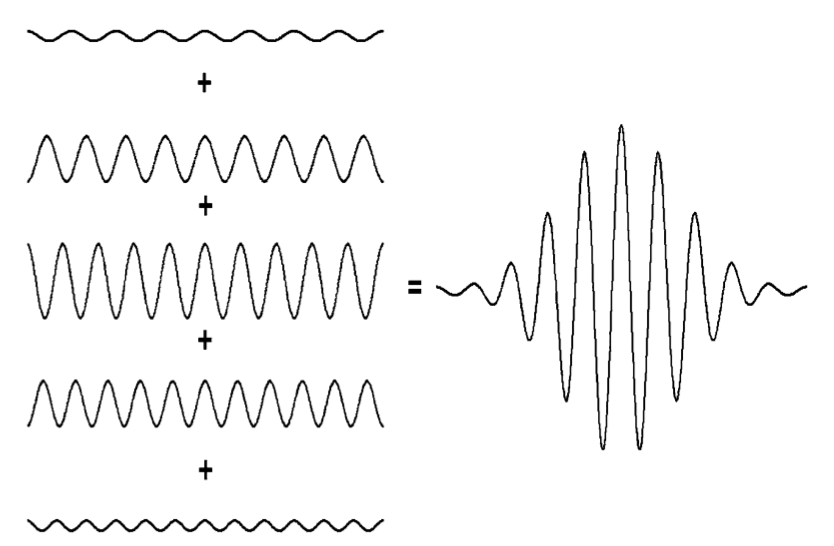
\includegraphics{figures/morgan_2}
\caption{“Combining interference signals from a range of wavelengths (left) produces a pulse (right). The width of this pulse determines the axial resolution of optical coherence tomography.” \cite{mbib_6} }
\label{fig:m_2}
\end{figure}

The pulse envelope’s width reveals the coherence length by providing
the coherence time (time of flight).  The coherence length can be found
by multiplying the time of flight by the speed of light, and is an
important quantity as it "determines the axial resolution of the OCT
system." \cite{mbib_6}  By scanning the retina and recording this
information, “the amplitude of reflected light can be plotted against
delay to demonstrate tissue reflectivity at successively deeper levels
of tissue penetration along the axis of beam propogation.” \cite{mbib_6}
These scans are known as A-scans.  The A-scans represent the reconstruction
of a plane “through the anterior or posterior segment of the eye.”\cite{mbib_6}
This reconstruction, illustrated in \fref{fig:m_3}, produces a “tomographic
image with an A-scan for each x and y location” and is called a B-scan and is
usually a grey-scale image for diagnostic purposes as the pseudo color images
make it hard to distinguish details that are easy to miss. \cite{mbib_5,mbib_4,mbib_7} 

\begin{figure}[htbp]
\centering
 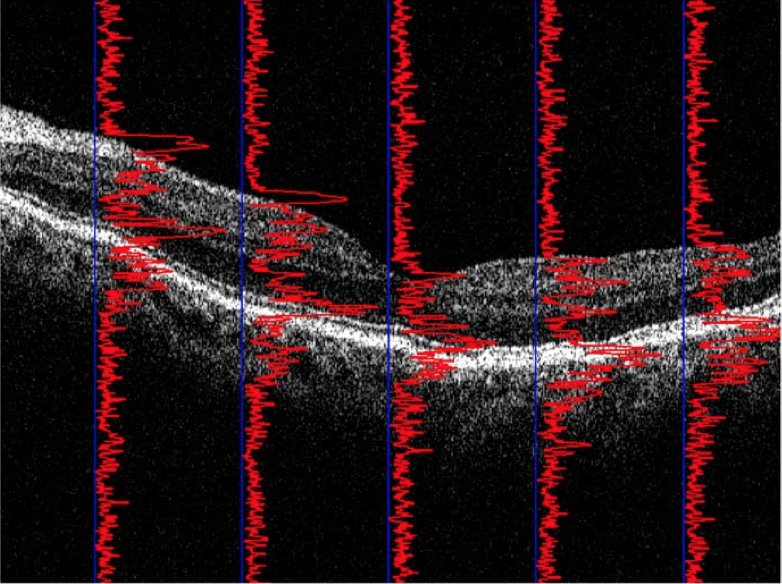
\includegraphics{figures/morgan_3}
\caption{“An optical coherence tomography cross-sectional image (gray- scale image) is built up from many A-scans (red plot lines).” \cite{mbib_6} }
\label{fig:m_3}
\end{figure}


The above description is how Time-domain OCT utilizes low coherence interferometry.
The other option is having a fixed reference mirror and attaching a spectrometer to
the detection arm to record the spectral signal from the reflected “bursts” of light,
which is known as Spectral-domain OCT.\cite{mbib_3} The next section will go into
more detail on the different imaging methodologies.

\section{Time-Domain and Spectral-Domain Optical Coherence Tomography}
Time-domain and Spectral-domain Optical Coherence Tomography differ in the way
the backscatter of the light from the super-luminescent diode from the retinal
tissues is analysed.  To briefly describe the differences between the two main
methods: TD-OCT resolves depth by measuring its flight time through the retina,
whereas SD-OCT uses a spectrometer to "measure the difference in wavelength
between the light from the fixed reference arm and that [of the light] returning
from the tissue" to generate these cross-sectional images.\cite{mbib_7} 

In both cases, the light wave travels through the retina as illustrated in Figure
4 and is reflected from each layer (detailed image of these layers can also be
found in \fref{fig:m_4} ) because the layers have different refractive indices.
Thus the backscatter of the light from “deeper tissues can be differentiated from
backscatter originating at more superficial tissues because it takes longer for
the light to arrive at the sensor;” a physical principle utilized
in Time-domain OCT imaging.\cite{mbib_4}

Time-domain OCT is when the reference mirror is mechanically moved to different
positions using the galvanic mirrors with freedoms in the x and y directions,
resulting in a time difference between the light from the reference arm and the
light returning from the retinal tissues.  These time differences depend on the
depth at which the light is backscattered from and can be used to reconstruct
retinal structure.  Since the speed at which the mirrors can be moved is limited
mechanically, “only thousands of A-scans can be obtained per second.” \cite{mbib_4}

\begin{figure}[htbp]
\centering
 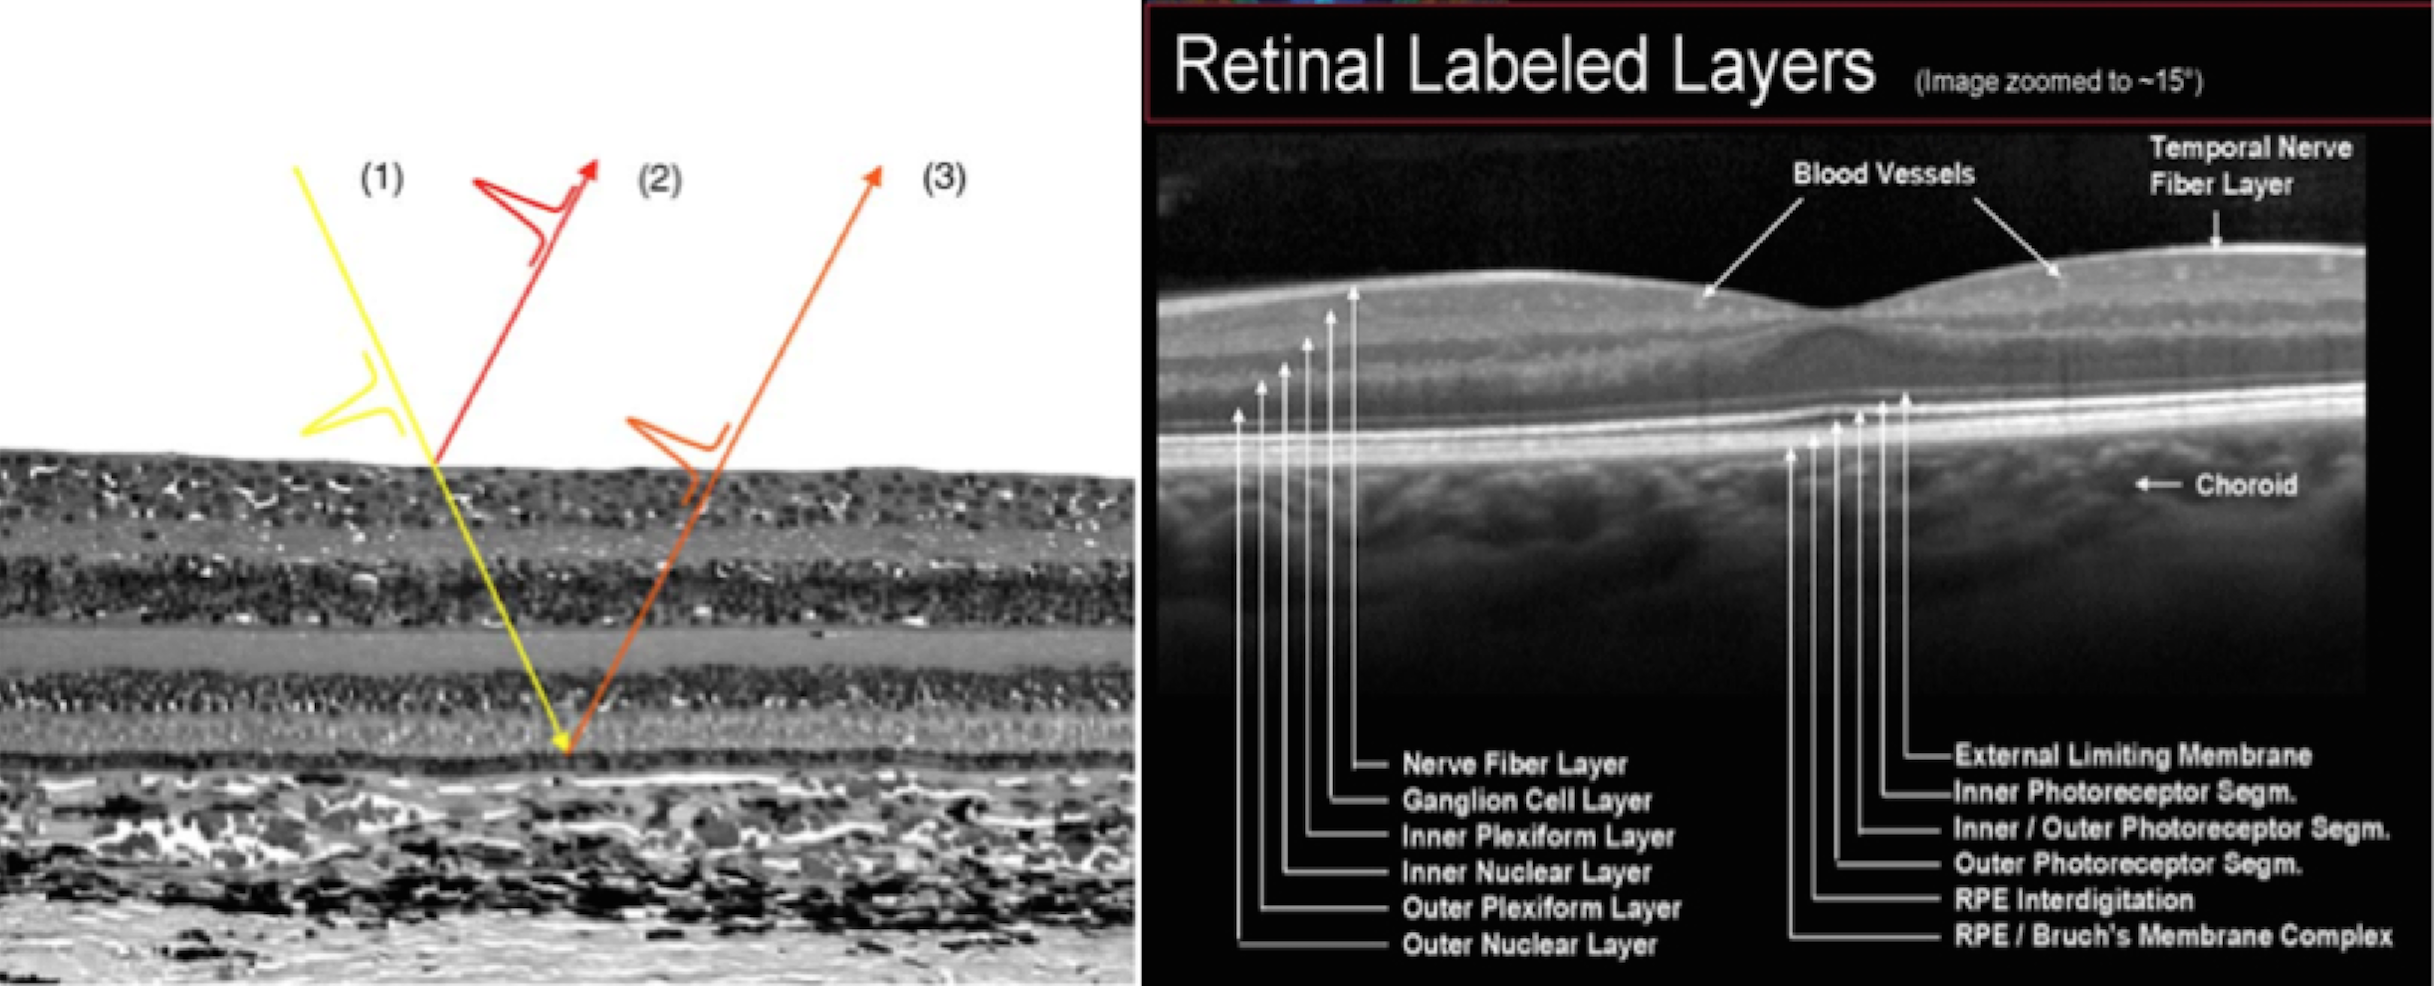
\includegraphics{figures/morgan_4}
\caption{(Left) "The optical coherence tomography beam is scanned across the retina (1).
The delay of a superficial reflection (2) is shorter than that of a deeper reflection (3)" (Right) A two dimensional black and white SD-OCT scan with an image zoom of 15$^\circ$.\cite{mbib_6}  This scan shows the retina with retinal
tissue layers labelled using arrows to give meaning to the image.\cite{mbib_8} }
\label{fig:m_4}
\end{figure}

Another physical principle that is utilized in Spectral-domain OCT imaging is the
fact that the reflected light will have a different spectral fingerprint than the
initial light sent into the eye which will return from the reference arm.  Instead
of continuously moving the reference arm, as in TD-OCT, the reference arm is kept fixed. 

The main difference between Fourier-domain and Spectral-domain OCT is that in FD-OCT
the “light source is rapidly modulated over its center wavelength” providing another
tag to the light; whereas in SD-OCT “a broadband light source is used,” and the signal
from the interferometer is spectrally decomposed using a diffraction grating and a CMOS
(Complimentary Metal Oxide Semiconductor) or CCD (Charged Coupled Device) linear sensor.\cite{mbib_4}
Thus a spectrometer is used to detect the spectrum created by the backscatter to produce
an image of the retina.  Once the signal is obtained a Fourier transform (“mathematical
procedure that extracts the frequency spectrum of a signal”) is applied to the spectral
signal to determine the depth of all “tissue scatters” at the x and y coordinates.\cite{mbib_4,mbib_9}
SD-OCT technology can provide “greater resolving power of the retinal layers, significantly
higher scan density, and faster data acquisition than original TD-OCT.” \cite{mbib_2}

\section{Images}
A-scans and B-scans were mentioned previously at the end of the low coherence interferometry
section.  For many years two dimensional B-scans were the highest achievable image possible
because OCT technology could not take images fast enough to acquire enough images to
construct a three dimensional image of the retina.  Due to patient comfort, and safety
requirements limiting how much light can be projected onto the retina, images can only be
taken for 1-3 seconds. \cite{mbib_4} With the improvement of SD-OCT, hundreds of thousands
of A-scans can be taken a second as opposed to the 400 A-scans a second achieved by
commercially available TD-OCT machines; making three dimensional images of the retina
possible.\cite{mbib_4}  Three dimensional images are now widely used in the clinical
setting as a standard of care.  As the technology improves, increasing the number of
A-scans taken in a second, higher resolution can be achieved in 3-D image volumes.\cite{mbib_4}

The overall resolution of these images in the x and y directions is dependent on the
speed and quality of the galvanic mirrors used in TD-OCT.  In the z direction the
coherence of the light limits the resolution.  Both of these limitations were mentioned
previously in the section describing the methods of analysing the returning light
backscatter from the eye.

Ultimately OCT imaging technology is looking for a way to achieve isotropic images
of the retina, meaning the size of each element imaged is the same in all three
dimensions.  OCT devices commercially available currently can only achieve images
isotropic in the x-y plane, and “offer voxel sizes of 30 × 30 × 2 μm.” \cite{mbib_4}
This is because current OCT technology always has higher resolution of depth than
in the x-y plane. \cite{mbib_4}  Although a completely isotropic is not possible
with current technology, there is an advantage to having “x−y isotropic imaging”.\cite{mbib_4}
It reduced the number of assumptions that have to me made of the retinal tissues
between the measures samples when analysing the images taken and quantifying
properties of the retina for medical purposes. \cite{mbib_4} This helps
ophthalmologists add more accurate images to the collection of information
making up retinal morphology.

Although the images are of high quality and resolution, the practitioner must consider
some other limitations.  For example corneal conditions such as dry eye, blinking, and
dilation of the eyes.  To tackle these limitations: dry eye can be addressed by applying
artificial tears to the patient’s eyes prior to the examination; blinking can be prevented
by shortening the scanning time and having the patient focus on the stimulus ("a cross of
green segments similar to a star"); and in order to achieve a larger scan of the retina,
many practitioners dilate the patients eyes as in many other retinal imaging examinations.\cite{mbib_4}

\section{Medical Applications of OCT}
OCT has many biomedical applications, however, the chief among them is retinal imaging
and is particularly useful for "identifying, monitoring and quantitatively assessing" retinal
diseases.\cite{mbib_9,mbib_4, mbib_5}  Before OCT there was very little information in
the database of retinal morphology.  With OCT imaging this database has grown, providing a
“wealth of new information” and has enabled practitioners to closely monitor retinal
diseases and help guide them in the treatment of patients with existing problems for
therapeutic purposes.\cite{mbib_4} 

“Currently, OCT imaging is widely used to determine the extent and amount of retinal thickening”
to help monitor these treatments, as well as the progress of the treatment post operation.
This is done by imaging the thickness of the retinal tissue layers to find areas where a
retinal layer is thicker than the rest of that layer in the rest of the retina.  Retinal
layer thickness is the most common property currently utilized by medical professionals
in the tracking and diagnosing of retinal diseases, however, other properties can be looked
into such as analyzing the images for textural properties in each of the layers, and quantifying
fluid parameters. \cite{mbib_4}

\section{Diabetic Macular Edema (DME)}
The most common application is in diabetic macular edema (DME). A patient with DME  leaks
fluid in the macula which in turn causes visual loss in said patient.  An original research
paper titled Early Treatment in Diabetic Retinopathy Study demonstrates that early treatment
of patients with DME with a focal laser can prevent further visual loss when targeting the
thickened areas of the retina. \cite{mbib_4}  This is done by analysing the thickness of the
retina and determining if there is an area of a retinal layer that is thicker than the rest.
An example of an OCT scan of someone with DME can be found in \fref{fig:m_5}. 

\begin{figure}[htbp]
\centering
 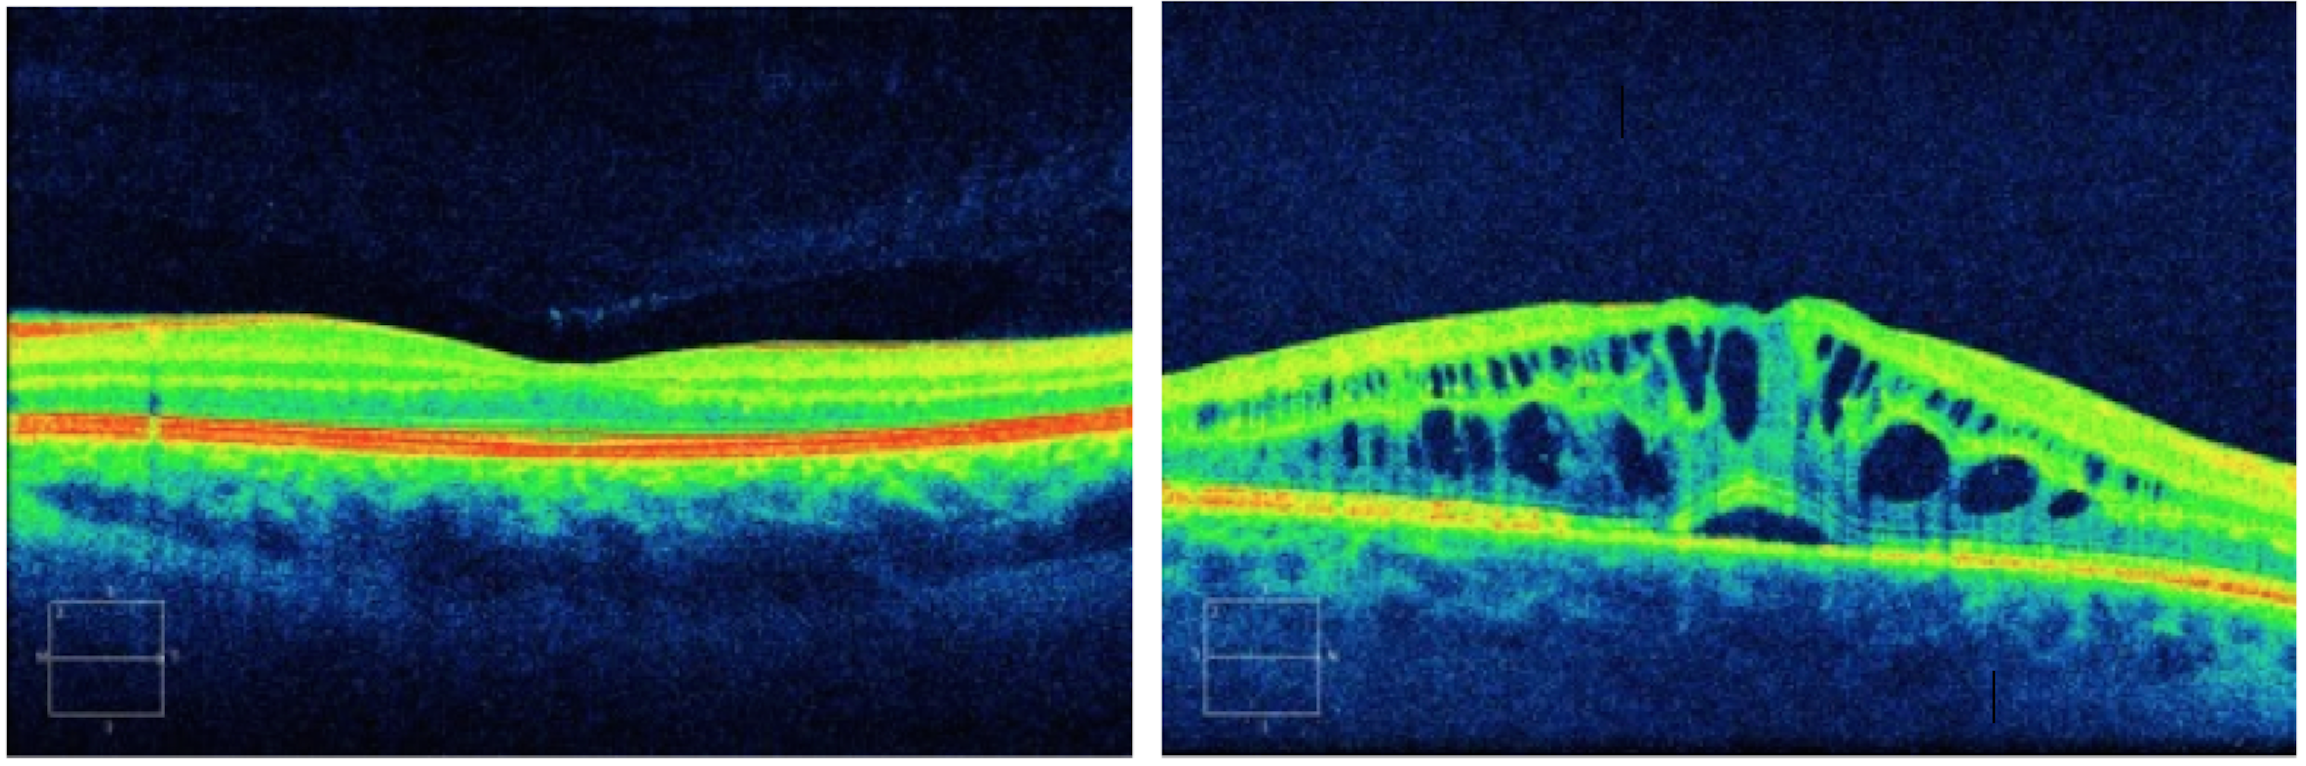
\includegraphics{figures/morgan_5}
\caption{Two images appear in this figure.  The left is an image demonstrating a patient with a normal retinal OCT scan in pseudo colors, while the left is that of a patient suffering from DME. \cite{mbib_10} }
\label{fig:m_5}
\end{figure}

\section{Glaucoma}
Glaucoma is a disease "characterized by gradual damage to the optic nerve and resultant visual
field loss."\cite{mbib_6} If diagnosed early this disease can be treated to reduce the risks of
vision loss.  Thus using OCT images to “observe a thinning of the retinal nerve fiber layer and
ganglion cell layer” is extremely useful in the treatment and management of glaucoma. \cite{mbib_4}
Both thickness and texture analysis of OCT images are useful in the care for patients with glaucoma.
Since the optic nerve is where glaucoma manifests, “the optic nerve head is an important structure
in the assessment of […] glaucoma.” \cite{mbib_4}  \Fref{fig:m_6} is an image of example optic nerve
OCT image analysis, comparing different methods of analysing the images.

\begin{figure}[htbp]
\centering
 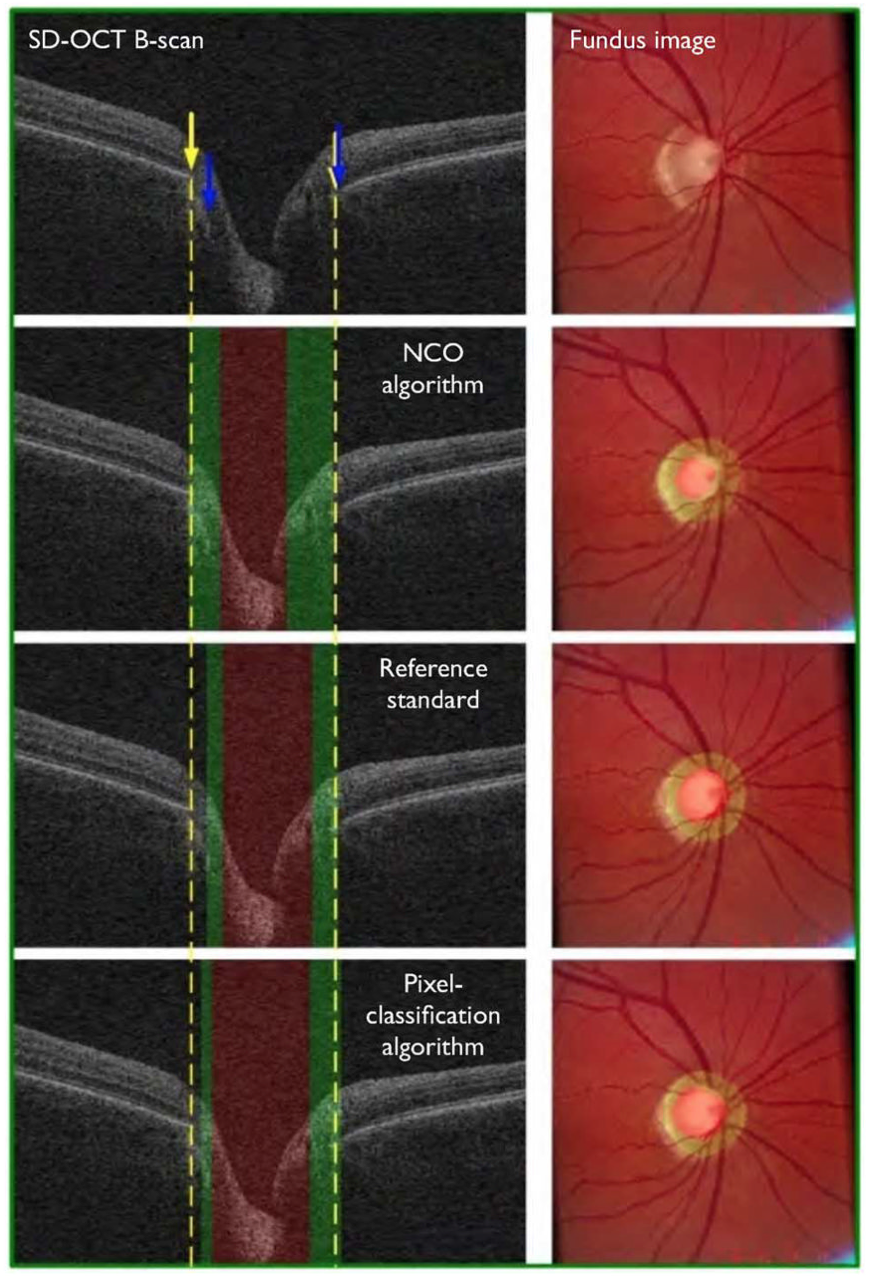
\includegraphics{figures/morgan_6}
\caption{This figure includes from top to bottom: a raw SD- OCT B-scan and corresponding
fundus image (top), structure-based (row 2), expert on fundus photography (row 3) and
pixel-classification-based (bottom) segmentations overlapping with raw SD-OCT and
corresponding fundus image.  From left to right: SD-OCT central B- scan (left) and
fundus image (right).  Yellow arrows indicate the position of the neural canal opening
(NCO) from algorithm (with dashed yellow line indicating projected NCO position).
Blue arrows indicate clinical disc margin from RS. Green and red colors indicate each
method’s projected rim and cup regions, respectively. \cite{mbib_4} }
\label{fig:m_6}
\end{figure}

\section{Symptomatic Exudate-Associated Derangements (SEADs)}
Another application of texture analysis application to retinal diseases, is using this
property along with layer-based properties to detect retinal lesions in both two and
three dimensional OCT images. Out of all of the different types of lesions, symptomatic
exudate-associated derangements (SEADs) are the prime interest “in assessing severity
of age-related macular degeneration, diabetic macular edema, and other diseases.”
\cite{mbib_4} Examples of these can be found in \fref{fig:m_7}

\begin{figure}[htbp]
\centering
 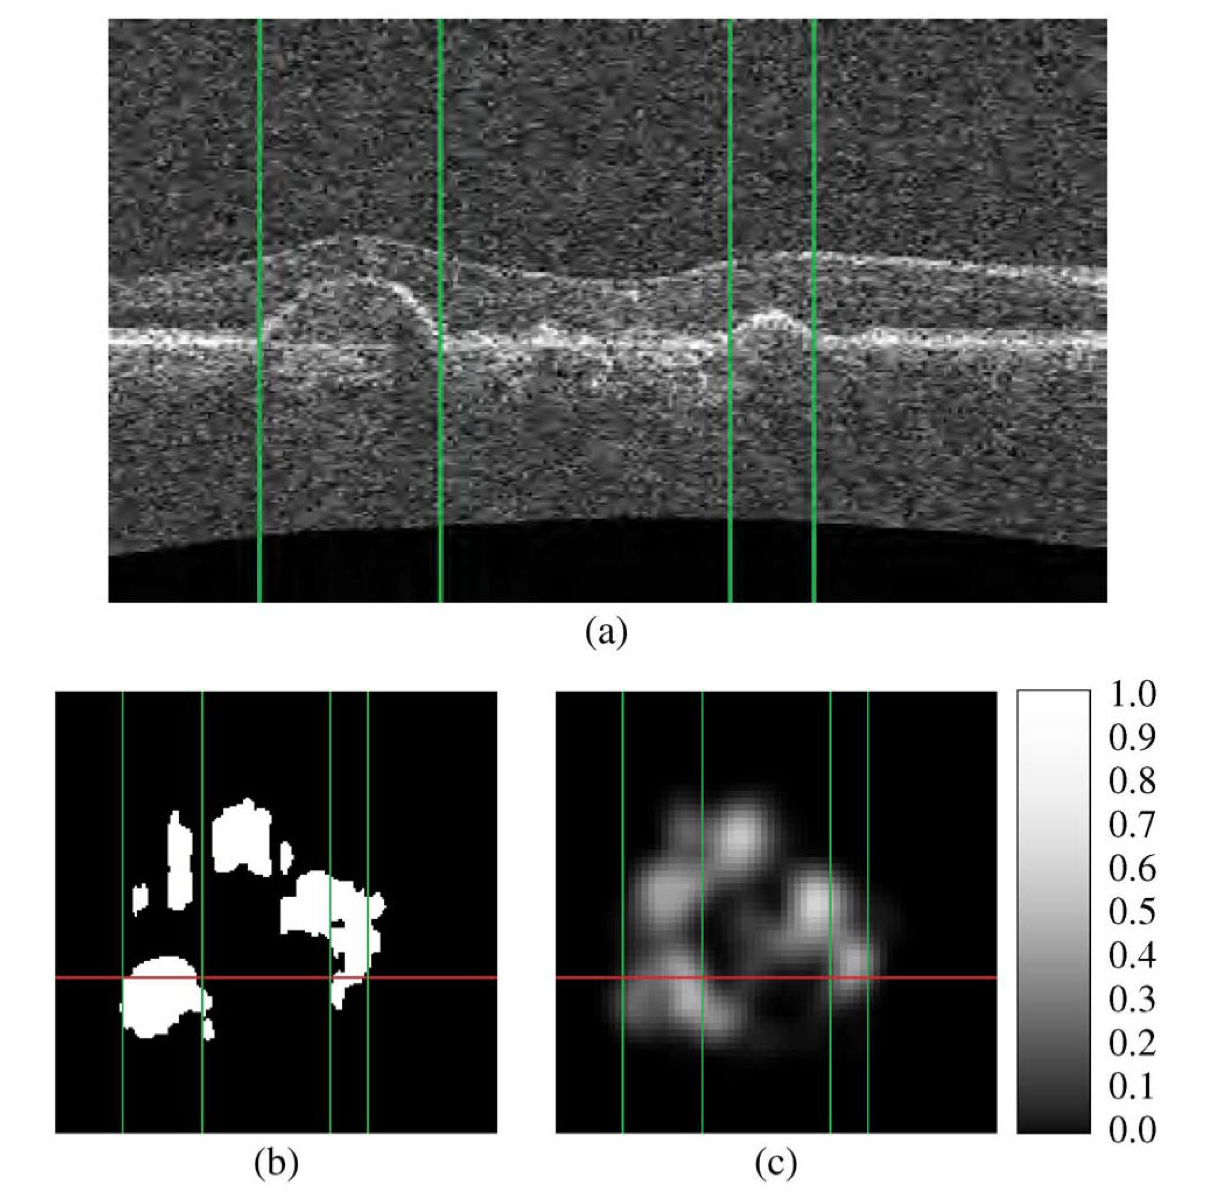
\includegraphics{figures/morgan_7}
\caption{“Example of SEAD footprint detection. Panel (a) presents an x − z slice running through SEADs in SD-OCT volume. Expert standards for footprint of these SEADs and automatically generated SEAD footprint probability map, in x − y plane, are presented in panels (b) and (c), respectively. Note probability scale in panel (c). Projection of x − z slice in x − y plane is represented by a vertical line in (b) and (c). Location of SEADs visible in panel (a) are indicated by vertical lines in each panel.” \cite{mbib_4} }
\label{fig:m_7}
\end{figure}

\section{Choroidal Neovascularization}
Choroidal neovascularization is another blinding disease know as “the wet form of age related macular degeneration,” and the main indicators of this disease are outer and sub-retinal fluid. \cite{mbib_4}  By using OCT imaging to quantify fluid parameters and affected retinal tissues in patients with this disease, proper treatment can be applied.\cite{mbib_4} \fref{fig:m_8} is contains an OCT scan of someone suffering from choroidal neovascularization.

\begin{figure}[htbp]
\centering
 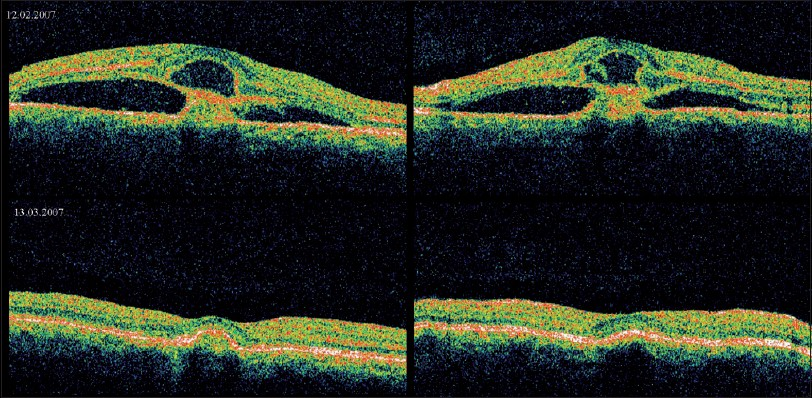
\includegraphics{figures/morgan_8}
\caption{ “Horizontal and vertical 6-mm line scan Optical coherence tomography images show sub-foveal choroidal neovascular membrane associated with sub-retinal fluid and cystoid macular edema at baseline (first row). Repeat Optical coherence tomography scans show disappearance of cystoid edema and complete resolution of sub-retinal fluid at one-month follow-up (second row)” \cite{mbib_11} }
\label{fig:m_8}
\end{figure}

\section{Further Improvements}
The current state of OCT technology can already achieve much more than the
original technology developed in 1991 could.  Previously unachievable
capabilities of these machines are now clinically standard practice in the
medical diagnosis of several retinal diseases.  Although these improvements
are highly effective in improving the technology for retinal imaging, further
research can be done to obtain images of deeper structures within the eye such
as “the choroidal vessels” which are a structure in the optic nerve and
relevant to “glaucomatous damage.” \cite{mbib_4}  Current commercially available
machines use wavelengths around 840$\mu m$ and only allow medical professionals
to image the retina.  Longer wavelengths around 1000-1300 $\mu m$ would enable
the OCT imaging light to penetrate deeper into the tissue and image these deeper
structures. \cite{mbib_4}
